\documentclass[10pt,a4paper]{article}
\usepackage{tikz} % for drawing figures
\usepackage{amsmath} % for equations
\usepackage{url} % for URLs
\usepackage{graphicx}
%\usepackage{float}
\usepackage{multicol}
\usepackage{varwidth}
\usepackage{blindtext}


\usepackage{linguex} % ** special include in directory: for doing handy example labeling and bracketing
\renewcommand{\firstrefdash}{} % used for linguex package not to put hyphens in example refs (1a instead of 1-a)
\usepackage{cogsci}
\usepackage{pslatex}
\usepackage{apacite}

\newcommand{\sem}[1]{\mbox{$[\![$#1$]\!]$}}
\newcommand{\lam}{$\lambda$}
\newcommand{\gcs}[1]{\textcolor{blue}{[gcs: #1]}} 
\newcommand{\lsp}[1]{\textcolor{violet}{[lsp: #1]}} 
\newcommand{\kj}[1]{\textcolor{green}{[kj: #1]}} 
%kj: These are great commands!
%LSP: Right? Greg for the win!

%% LSP: woohoo, git change
%%KJ: Another test git change!


\title{Modeling scope ambiguity resolution as pragmatic inference:\\ 
Formalizing differences in child and adult behavior}
\author{\large \textbf{K.J. Savinelli}, \textbf{Gregory Scontras}, and \textbf{Lisa Pearl}\\
\{ksavinel, g.scontras, lpearl\} @uci.edu\\
University of California, Irvine}


\begin{document}
\maketitle

\begin{abstract}
Investigations of scope ambiguity resolution suggest that child behavior differs from adult behavior, with children struggling to access inverse scope interpretations. For example, children often fail to accept \textit{Every horse didn't succeed} to mean not all the horses succeeded. Current accounts of children's scope behavior involve both pragmatic and processing factors.
%\cite{MuLid2006, gualmini2004some, gualmini2008rise, viau2010priming}. 
Inspired by these accounts, we use the Rational Speech Act framework to articulate a formal model that yields a more precise, explanatory, and predictive description of the observed developmental behavior.


\textbf{Keywords:} 
Rational Speech Act model, pragmatics, processing, language acquisition, ambiguity resolution, scope

\end{abstract}

\section{Introduction}

%LSP: Just focus on the scopal ambiguity first
If someone says ``\textit{Every horse didn't jump over the fence}," do you think any horses made it over the fence? If you think not, then you've interpreted this utterance as something like  
%``\textit{\textbf{No} horses jumped over the fence}''. 
\ref{ex:surface}.
In contrast, if you think it's possible some horses made it, you've interpreted this utterance as something like 
%``\textit{\textbf{Not all} the horses jumped over the fence}''. 
\ref{ex:inverse}.
These two different interpretations are possible because the utterance is  scopally ambiguous. That is, it contains two scope operators: a quantifier (\textit{every}=$\forall$) and a negation (\textit{n't}=$\neg$).  Either element can take scope over the other (indicated as $>>$ in \ref{ex:scope-ambig}), and so yield two different interpretations. 

\ex. \label{ex:scope-ambig} \textit{\underline{Every} horse did\underline{n't} jump over the fence}.
\a.  \label{ex:surface} $\forall>>\neg$ (surface scope): \\
\textbf{None} of the horses jumped over the fence.
\b.  \label{ex:inverse} $\neg>>\forall$ (inverse scope):\\ 
\textbf{Not all} of the horses jumped over the fence.

While adults can access both interpretations given appropriate context,  5-year-old children typically struggle to obtain the inverse scope in \ref{ex:inverse} \shortcite{Muso1998, lidz2002children,MuLid2006,musolino2006structure,viau2010priming,tieu2015isomorphism}.  For example, in a context where two out of three horses did in fact jump over the fence, only the inverse scope interpretation in \ref{ex:inverse} is true. 
%\gcs{if we're pressed for space, I would cut down on the discussion that follows (i.e., the principle of charity and QAR -- they don't play much into our investigation)}
Adults 
%obey what's been called the \textit{Principle of Charity} \cite{gualmini2004some}, 
charitably interpret the ambiguous utterance in a way that makes it a true statement (i.e., with the inverse scope in a two-out-of-three scenario), but  5-year-olds 
%The reluctance of five-year-olds to judge the sentence as true in such a scenario leads to the observation that children do \emph{not} adhere to the Principle of Charity, instead %seem to resolutely 
stick with the surface interpretation in \ref{ex:surface}, which is false. Why does children's behavior differ from adults' in this context?

%% so let's talk about the previous accounts of children's behavior: processing and pragmatics
Previous accounts of children's scope interpretation behavior have recognized that both processing and pragmatic factors may contribute to non-adult-like behavior.
%% processing first
\citeA{Muso1998,musolino2006structure} observed that the surface scope  interpretation in \ref{ex:surface} may be easier to process because  the scope  relationship in the semantics (i.e., $\forall$ scopes over $\neg$) aligns with the  linear order of these elements in the utterance (i.e., \textit{Every} precedes \textit{n't}). In contrast, for the inverse scope interpretation in \ref{ex:inverse}, this isomorphism does not hold,  with the scope relationship (i.e., $\neg$ scopes over $\forall$) opposite the linear order of the elements in the utterance. Musolino hypothesized that this lack of isomorphism would make the inverse scope interpretation more difficult to access. 
% A listener would need to do an extra step in parsing the utterance to get to that semantic representation from the surface form.
% In support of this explanation, one experiment suggests that adults favor the surface scope when their interpretation of a scopally ambiguous utterance like (1) is time restricted \cite{conroy2008surface}.
In line with this prediction, 
\shortciteA{conroy2008surface} found that when adults are time-restricted, they favor the surface scope interpretation. 
%of ambiguous utterances. 
We thus see a potential role for processing factors in children's inability to access the inverse scope. Perhaps children, with their still-developing processing abilities, can't allocate sufficient processing resources to reliably access the  %non-isomorphic  %LSP: we should  pick one term (inverse or non-isomorphic) and stick with it, I think
inverse scope interpretation.

%% but there are also pragmatic factors
In addition to this processing factor, \shortciteA{gualmini2008question} noted that discourse properties, such as what children consider the 
%topic or 
\textit{question under discussion} (QUD), 
may impact their scope interpretation behavior.  Formal theories of pragmatics suggest that all discourse transpires with respect to some QUD, whether implicit or explicit; utterances in the discourse need to (at least partially) answer the QUD to be pragmatically felicitous \cite{roberts2012information}. Gualmini and colleagues \shortcite{hulsey2004question, gualmini2008question} suggest that children are very sensitive to this requirement.
%, terming it the \textit{Question-Answer Requirement}. 
% relationship to processing??
%The principled idea being that relevant utterances are easier to process (Sperber citation?).
In particular, children may be able to access the inverse scope interpretation but nonetheless choose the surface scope interpretation because it better answers the perceived QUD in the contrived experimental setups.  
%Gaulmini (2008) claims that the Question-Answer requirement might be a higher ranking constraint on utterance interpretation than the principle of charity.
%  Children differ from adults in this account, not because of a difference in grammatical competence or parsing limitations, but because of a still developing pragmatic competence; i.e. the lack of ability to generate or infer the proper QUD, or to compute the scalar implicatures that would be necessary to arrive at an interpretation that answers the QUD.
So, children's observed behavior would derive from a still-developing ability to manage the contextual information available and correctly infer the intended QUD.

Thus, children's developing processing and pragmatic abilities may both be a source of the observed non-adult-like behavior \cite{viau2010priming},
% but it's muddy right now...better way to say this?
though current experimental studies have struggled to clearly isolate the influence of each type of factor.
%% so that's where we come in
To this end, we formally articulate the mechanism of scope ambiguity resolution using the Bayesian Rational Speech Act (RSA) computational modeling framework \shortcite{frankgoodman2012,goodmanfrank2016} %LSP: We should cite Noah's stuff.
%  It also offers us a computational framework from which to understand exactly how the variables considered here would impact a scopally ambiguous utterance's endorsement.
in order to identify the separate contributions of processing and pragmatic factors.

% So here's what we're going to do in the rest of the paper to accomplish that
We first summarize key experimental results from the literature on child scope ambiguity resolution, noting three core variables (one processing, two pragmatic) that affect children's scope disambiguation behavior. We also highlight the nature of the task children are being asked to engage in, 
% precise
which we then formally articulate using an RSA model that specifies the role of each of these three variables.
Our results suggest that pragmatic factors play a larger role than processing factors in explaining children's non-adult-like scope ambiguity resolution behavior, 
% explanatory
and the computational modeling framework allows us to understand exactly why that's so. %\lsp{Do we want to hint at the big picture idea of why that's so?}\gcs{I think we should save it}
% predictive
These results additionally suggest targeted future behavioral experiments to verify the impact of the specific pragmatic factors we identify.  
% sum it up, like in the abstract
More generally, our model yields a more precise, explanatory, and predictive description of the observed developmental scope ambiguity resolution behavior.


\section{Background: Experimental results}

%LSP:  Going directly to the heart of it.
Children's ability to access the inverse scope interpretation has been shown to be sensitive to manipulations of experimental context.
% about the task that's used 
The methodology typically used to assess children's scope disambiguation is the Truth Value Judgment Task (TVJT; \citeNP{crain1985acquisition}).  In the basic TVJT, children are presented with a background story about the actors---for example, horses engaging in some activities.  After this background story, children watch as the horses attempt to complete an action, such as jump over a fence. 
%TVJTs typically have a many of horses succeed and a few horses (typically one) fail.  
The critical \textbf{not-all} result state meant to prompt the inverse scope interpretation is illustrated in Figure \ref{fig:horse}, where the white horse fails to jump over the fence. 

\begin{figure}[!ht]
\begin{center}
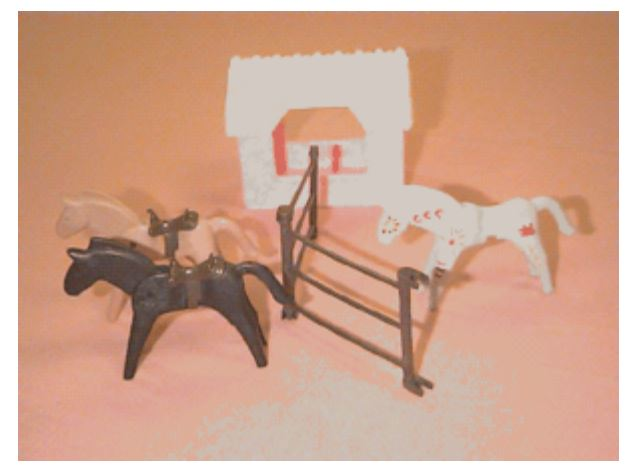
\includegraphics[width=50mm,scale=0.5]{musolidz_horses_pic.JPG}
\caption{Sample \textbf{not-all} scenario from \citeA{MuLid2006}: 2 of 3 horses succeed at jumping over the fence.}
\label{fig:horse}
\end{center}
\end{figure}

In this scenario, the surface scope interpretation of the scopally-ambiguous utterance \textit{Every horse didn't jump over the fence} (i.e., \textbf{none} of the horses jumped over the fence) is false,  and the inverse scope interpretation (i.e., \textbf{not all} of the horses jumped over the fence) is true.  A puppet then says the scopally-ambiguous utterance, and the child is asked to state if the puppet is right. %spoke true
% just to make the endorsement link early
That is, the child is asked  whether s/he would endorse the puppet's utterance as a true description of the scenario.
%They are then asked to justify their answers. 
Typically, children  refuse to endorse the puppet's utterance, saying that the puppet is wrong.
 This behavior has been interpreted as children failing to access the inverse scope interpretation that would make the utterance true.
%It is in this `basic' version of the TVJT that we see the behavioral differences between adults and children.

%What about this task needs to change in order for children to endorse the ambiguous utterance in a not-all scenario?
% Here we review three alterations to the basic TVJT paradigm that yield more adult-like behavior in children. 
Interestingly, various alterations to the TVJT setup have yielded more adult-like behavior in children, namely greater rates of endorsing the puppet's ambiguous utterance in {not-all} scenarios.
% Musolino & Lidz 2006: early-success expectations + affirmative action 
% LSP: I checked Viau et al. 2010 and found that M&L2006 actually did both of these together and it's Viau et al. 2010 who deconfounded them and found that either will do for increasing utterance endorsement
\citeA{MuLid2006} observed that negation in an utterance might require certain felicity conditions to be met. In particular, negated utterances require a preceding \textit{affirmative context} to contrast with \cite{wason1965contexts}.  
\citeauthor{MuLid2006} augmented the basic TVJT to include an additional contrast condition in which the puppet precedes its negative scopally-ambiguous utterance with a contrasting affirmative clause. This additional clause describes a previous successful story action (i.e., \textit{early-success}),  such as  \textit{Every horse jumped over the log, but every horse didn't jump over the fence}. 
This early-success contrast manipulation increased children's willingness to accept the scopally-ambiguous utterance in the {not-all} scenario: Children in the baseline condition endorsed the puppet's statement just 15\% of the time, while children in the
% just to use the same term highlighted above
early-success affirmative context
condition endorsed the puppet's statement 60\% of the time. 
\citeA{viau2010priming} later replicated this 
%increased utterance endorsement based solely on the presence of earlier success in the story context.
increase in utterance endorsement using only an early-success story context. 
%That is, even  with this affirmative context information only in the pragmatic context and not explicitly in the utterance to be endorsed, children maintained the increased endorsement rate.
That is, the utterance endorsement rate was maintained by an early-success story context alone, and children didn't need an explicit contrast clause in the test utterance.

%increased to 60\% with only a preceding story element indicating success (e.g., all horses jumping over a log)---i.e., without the linguistic affirmation statement preceding the utterance. \gcs{not sure I understand this -- the utterance to be endorsed is the simple mono-clausal ambiguous one, but they witness early success without hearing it described?}


Notably, the early-success affirmative context manipulation  potentially changes several aspects of the experimental context.  
% To wit, participants are given information about the horses' jumping ability, potentially increasing expectations for jumping success.
First, it can shift participants' \textit{expectations} about successful outcomes in the experimental world.
% Moreover, the early-success utterance could increase the salience a QUD that targets this success, something along the lines of ``did all of the horses succeed?'' As we shall see, both of these changes to the context can potentially shift behavior on the TVJT.
This shift then potentially increases the salience of a {QUD} targeting this success, such as \textit{``Did all the horses succeed?''} (\texttt{all?}). 
Recognizing this QUD's potential significance, \citeA{gualmini2004some} attempted to manipulate the experimental context so it favored the \texttt{all?}~{QUD}.
%%LSP: Just checked Gualmini 2004. He actually manipulated the implicit QUD by manipulating the story context. (ex: the story is all about trolls delivering pizzas, not losing pizzas. Therefore, QUD is about success at delivering, not at losing.)
%  "The troll didn't deliver some pizzas." <-- 90% endorsement when 2 delivered and 2 not delivered
With \texttt{all?}~as the salient QUD, children's endorsement of a scopally-ambiguous utterance that perfectly answers \texttt{all?}~in the critical {not-all} scenario increased to 90\%.  
Even for a scopally-ambiguous utterance that does \textit{not} answer the \texttt{all?} QUD, children's endorsement rate was at 50\%---markedly higher than the 15\% baseline from the original study by \citeA{MuLid2006}.
%\gcs{I wonder if the above suffices as a summary of Gualmini (i.e., if less is more)}
%LSP: works for me
% what this means: QUD matters 
This finding highlights that privileging the \texttt{all?} QUD increases children's utterance endorsement in these scenarios.
 

% GCS: moved old text to the "extra bits"

%% scope interpretation priming is also tied up with this
A third potential impact of the affirmative context manipulation involves scope access.
By  altering the experimental world expectations and/or QUD to increase access to the inverse scope, the inverse scope interpretation may also become more accessible for later use.  \citeA{viau2010priming} term this \textit{structural priming}.  
% relate this to utterance endorsement
Children who are better able to access the inverse scope are then more likely to endorse the scopally-ambiguous utterance in subsequent {not-all} scenarios.
\citeauthor{viau2010priming} investigated structural priming explicitly by attempting to 
directly alter the accessibility of the inverse scope interpretation. %, focusing on the grammatical operations children use to derive the inverse scope interpretation.
In one modified TVJT, they attempted to prime the access of the inverse scope interpretation, and in another modified TVJT, they attempted to directly prime the inverse scope's logical structure (e.g., $\neg>>\forall$).

%[manipulation 1: first three trials are early-success context = increases utterance endorsement; later three trials are early-failure context% ]
%[effect 1: endorsement at 80\% for early-failure context after early-success previous contexts ]
The first structural priming manipulation was implemented via the now-familiar %early-success 
affirmative context (i.e., pragmatic) manipulation. For the first three trials, the  prior experimental context indicated successful outcomes and the effect was that children endorsed the scopally-ambiguous utterance 50\% of the time. Crucially, the subsequent three trials removed the supportive affirmative context manipulation---yet children continued to not only endorse the scopally-ambiguous utterance, but to endorse it more than they had before (80\%).  
\citeA{viau2010priming} attribute this result to a priming effect of the inverse \emph{interpretation} from the first three trials. 
%[interpretation 1: expectations about the world matter and help to access inverse scope (perhaps by also manipulating the salient QUD) which leads to utterance endorsement, and utterance endorsement persists even after world context no longer is early-success. Why? Because access to the inverse scope is easier and/or QUD: all-succeed? has been primed.]
Interestingly, the increase in utterance endorsement could be due to priming multiple  factors that are products of the affirmative context manipulation:
% let's highlight how these things are intertwined
(i) the expectations about successful outcomes in the experimental world, 
(ii)  the salience of the \texttt{all?} QUD, or
(iii)  the ease of access to the inverse scope interpretation. 
  
%[manipulation 2: first three = early-failure context + unambiguous utterance (e.g., ``Not every horse jumped over the fence''; last three = early-failure context + ambiguous utterance (``Every horse didn't jump over the fence'') ]

The second structural priming manipulation removed the affirmative context story in the first three trials. 
% element so that the prior experimental context indicated horses failed at jumping) and so removed that supportive pragmatic factor. 
In its place, children were asked whether they would endorse a scopally-\textit{unambiguous} utterance (e.g., \textit{``Not every horse jumped over the fence''}) whose interpretation had logical operators in the same order as the inverse scope interpretation of the scopally-ambiguous utterance (e.g., $\neg>>\forall$).
% [effect 2: 80\% endorsement for all early-failure context both with unambiguous and ambiguous utterances]
Children endorsed this utterance 80\% of the time.
In the subsequent three trials, children were asked if they would endorse the scopally-ambiguous utterance in the same experimental scenario---and their endorsement rate remained at 80\%. 
%% [interpretation 2: inverse scope interpretation (=logical form $\neg>>\forall$ every) primed by unambiguous utterance, and persists. Why? Scope can matter on its own for endorsing the utterance. Or...by saying "Not all the horses succeeded", make QUD:all-succeed? more salient.]
\citeA{viau2010priming} interpret this effect as priming of the relevant logical form: The inverse scope was easier to access in the scopally-ambiguous utterance because it was so recently accessed in the unambiguous utterances. The authors argue that this priming effect proceeded in the absence of manipulations to the pragmatic context, 
%; so, utterance endorsement increased, even without supportive pragmatic context.
yet even here, there may still be pragmatic factors at work. 
% why?
The unambiguous utterance accomplishes three things: (i) it provides an instance of the $\neg>>\forall$ configuration, (ii) it provides information about successful outcomes, and (iii) it suggests the \texttt{all?}~QUD, answering it with \emph{no}. 
%because of the interplay between pragmatic factors and processing of the inverse scope. 
%More specifically, the unambiguous utterance (with its accompanying logical form) is a good answer to \textbf{QUD:all-succeed?}, i.e.,   ``\textit{Not all the horses succeeded}'' indicates the answer to \textit{Did all the horses succeed?} is \textit{no}.
Thus, in this attempt to prime the inverse logical form, the authors may have also altered expectations about the pragmatic context of the experiment, as related to the successful outcomes and relevant QUDs.
%salience of the pragmatically supportive QUD is also primed.   

%%% point: these things are hard to tease apart
These experimental studies highlight at least three core factors (two pragmatic, one processing) that  underlie children's utterance endorsement behavior in the TVJT:  
(i)  pragmatic: expectations about the experimental world (e.g., how likely successful outcomes are),
(ii) pragmatic: expectations about the QUD (e.g., 
%%LSP: Just to keep it simple, given that we've been priming the all? QUD throughout this section
%whether we're interested in the number of successful outcomes or 
whether all
%/no 
outcomes were successful), and
(iii) processing: the accessibility of the inverse scope (i.e., the ease by which the logical form is accessed). 
These experimental studies have also supported different theoretical proposals for the source of children's differences. The proposals split on whether they attribute the differences solely to an inability to manage contextual information (i.e., pragmatic factors; \citeNP{gualmini2008rise}) or whether processing deficits also significantly contribute (i.e., difficulty accessing inverse scope; \citeNP{viau2010priming}). Importantly, it is not obvious from any of the existing experimental manipulations how to separate the independent contributions of these components. To capture and independently manipulate the contributions of each of the pragmatic and processing factors, we formalize their role in the interpretation of scopally-ambiguous utterances, using tools from probabilistic modeling.


%Beginning of model section: we don't know which number corresponds to a behavioral result, and we don't know the value of these knobs for the individuals in the experiment.  Future experiment, getting knob values.  

\section{The model}

%give more information about what all the priors are, like exact values. More ecologically valid prior.  .7 and .3.  Put all the details in.

We model  ambiguity resolution within the Bayesian Rational Speech Act (RSA) framework \cite{goodmanfrank2016}. This framework views language understanding as a social reasoning process. A \textit{pragmatic listener} $L_1$ interprets an utterance by reasoning about a cooperative \textit{speaker} $S_1$ who is trying to inform a \textit{literal listener} $L_0$ about the world.
Our model is a ``lifted-variable'' extension wherein the ambiguous utterance's literal semantics is parameterized by interpretation-fixing variables (e.g., the relative scope of the quantificational elements; \citeNP{Lassiter2013}). Hearing an ambiguous utterance, a pragmatic listener reasons jointly about the true state of the world (e.g., how many horses jumped over the fence), the scope interpretation that the speaker had in mind (i.e., surface vs.~inverse), as well as the likely QUD that the utterance addresses (e.g., \texttt{all?}).  %LSP: Just to keep familiar nomenclature
%\emph{did all horses fail?}, \emph{did all horses succeed?}, \emph{how many horses succeeded?}
%This models the resolution of scope ambiguity as pragmatic inference over the parameters of an underspecified literal semantics, delivering quantitative predictions about behavior.
%as well as about the QUD and the scope interpretation that the speaker had in mind. 

% LSP: link to TVJT
To connect our model's predictions with the available TVJT data, we follow \citeA{degen2014lost} and \citeA{tessler2016manuscript}, modeling participants' TVJT behavior as the (relative) endorsement of  a \textit{pragmatic speaker} $S_2$ for an utterance about an observed situation. That is, we model whether a speaker would endorse the scopally-ambiguous utterance as a description of the observed state, or whether the speaker would prefer to say nothing at all.  
%\lsp{Do we want to mention a ``no'' option is somewhat equivalent to saying nothing at all (i.e., ``I do not want to endorse this utterance'')? Kids are usually asked to give a ``'yes'' or ``no'' answer in TVJT, with ``no'' presumably equivalent-ish to the ``I'd rather not say anything than endorse \textit{that} utterance'' option.} \gcs{I think where we've already translated the TVJT behavior into endorsement, this should suffice}
The pragmatic speaker $S_2$ makes this decision by reasoning about the probability that a pragmatic listener $L_1$ (who is reasoning about a speaker $S_1$ reasoning about a literal listener $L_0$) would arrive at the correct world state after hearing the utterance. 

We take world states $w\in W$ 
to correspond to the number of successful outcomes, for example, the horses that successfully jumped over the fence ($W=\{0,1,2,3\}$). We assume a simple truth-functional semantics where an utterance $u$ denotes a mapping from world states to truth values ($Bool = \{\texttt{true},\texttt{false}\}$). We parameterize this truth function so that it depends on the scope interpretation $i \in I = \{\texttt{inverse}, \texttt{surface}\}$,
\sem{\textit{u}}$^{i}$: $W\rightarrow$ Bool. 
We consider two alternative utterances $u \in U$: the \texttt{null} utterance (i.e., saying nothing at all, and so choosing \emph{not} to endorse the utterance) and the scopally ambiguous utterance \texttt{amb} (e.g., \textit{``Every horse didn't jump over the fence''}). So, $U$ = \{\texttt{null}, \texttt{amb}\}.  
The utterance semantics appears in \ref{ex:utt-sem},
% explain the difference for null vs amb
where the parameterization only impacts the truth value for utterance \texttt{amb} (since that's when multiple interpretations are available). 
% now explain about what surface and inverse do to the truth values
If \texttt{inverse} is active, this corresponds to the  \textbf{not all} reading, and so is true as long as not all (i.e., $w$$\neq$3) outcomes were successful.
If  \texttt{surface} is active, this corresponds to the \textbf{none} reading, and so is only true in world state 0.


\ex. \label{ex:utt-sem} \emph{Utterance semantics} \sem{\textit{u}}$^{i}$:
\a. \sem{\texttt{null}}$^{i}$ = \texttt{true}
\b. \sem{\texttt{amb}}$^{i}$ = \ \ \ \ if $i$ = \texttt{inverse}  \sem{\texttt{inverse}}, \\
\phantom{sem{\texttt{amb}}$^{i}$ = } else \sem{\texttt{surface}}\\
 where:\\
\sem{\texttt{inverse}} = $\lambda$w. w $\neq$ 3 \\
\sem{\texttt{surface}} = $\lambda$w. w = 0


We consider three QUDs $q \in Q$: 
(i) ``How many horses made it over?" (\texttt{how-many?}), 
(ii) ``Did all the horses make it over?" (\texttt{all?}), and 
(iii) ``Did none of the horses make it over?" (\texttt{none?}). 
The QUDs serve as projections from the inferred world state to the relevant dimension of meaning, $q: W \rightarrow X$ \shortcite{kao2014numbers,kao2014metaphor}. 
In practice, the QUDs establish partitions on the possible world states, as shown in \ref{ex:qud-sem}: 
% explaining this a bit more
\texttt{how-many?} is an identity function on world states, 
\texttt{all?} returns \texttt{true} only if  all three outcomes were successful, and 
\texttt{none?} returns \texttt{true} only if none of the outcomes were successful.


\ex. \label{ex:qud-sem} \emph{QUD semantics} \sem{\textit{q}}:
\a. \sem{\texttt{how-many?}} = \lam w. w
\b. \sem{\texttt{all?}} = \lam w. w = 3
\b. \sem{\texttt{none?}} = \lam w. w = 0


The literal listener $L_0$ has prior uncertainty about the true state, $P(w)$, and updates beliefs about $w$ conditioned on the the literal semantics.  That is, $L_0$ restricts prior beliefs to those worlds that $\sem{$u$}^i$ maps to \texttt{true}.  %LSP: Very helpful explanation!
The function $\delta_{[\![u]\!]^{i}(w)}$ maps the Boolean truth value to a probability, 1 or 0.

\begin{equation*}
P_{L_{0}} (w | u, i) \propto \ \delta_{[\![u]\!]^{i}(w)} \cdot P(w)
\end{equation*}
To capture the notion that communication proceeds relative to a specific QUD $q$, $L_0$ must infer not only the true world state $w$, but also the value of the QUD applied to that world state, $\sem{$q$}(w) = x$.
%infers the world state, computes the QUD

\begin{equation*}
P_{L_{0}} (x | u, i, q) \propto \ \sum_{w}\delta_{x=[\! [ q ]\! ](w)} \cdot P_{L_{0}} (w | u, i)
\end{equation*}

%\kj{to clarify for myself, the literal listener doesn't actually infer a qud, right?  Since there is no prior over quds here, the qud is just set when evaluating the probability for x}
% LSP: Right, that was my take on it. L_0 already knows what the QUD is when evaluating things because we're in literal semantics land.

The speaker $S_1$ chooses an utterance $u$ in proportion to its utility in communicating about the true state of the world $w$ with respect to the QUD $q$, $\sem{$q$}(w)=x$. Thus, the speaker maximizes the probability that $L_0$ arrives at the intended $x$ from $u$.
This selection is implemented via a softmax function ($exp$)  and free parameter 
$\alpha$, which controls how rational the speaker will be in utterance selection.  

\begin{equation*}
P_{S_{1}} (u | w, i, q) \propto  \ exp (\alpha \cdot log(L_{0}(x | u, i, q)))\\
\end{equation*}

Utterance interpretation happens at the level of the pragmatic listener $L_1$, who interprets an utterance $u$ to jointly infer the world state $w$, the interpretation $i$, and the QUD $q$. We therefore model \emph{ambiguity resolution} as pragmatic inference over an under-specified utterance semantics (i.e., the interpretation variable $i$). To perform this inference, $L_1$ inverts the $S_1$ model by Bayes’ rule, 
% explain what the equation terms are
and so the joint probability of $w$, $i$, and $q$ is proportional  to the  likelihood of $S_1$ producing utterance $u$ given world state $w$, interpretation $i$, and QUD $q$, as well as the priors on $w$, $i$, and $q$.
\begin{equation*}
 P_{L_{1}} (w, i, q | u) \propto  \ P_{S_{1}} (u | w, i, q) \cdot P(w) \cdot P(i) \cdot P(q)
\end{equation*}

To model the utterance endorsement implicit in TVJT, we need one more level of inference. The pragmatic speaker $S_2$ observes the true world state $w$ and selects $u$ by inverting the $L_1$ model, thus maximizing the probability that a pragmatic listener would arrive at $w$ from $u$
%LSP: explain how
by summing over possible interpretations $i$ and QUDs $q$ that accompany world $w$.

%\lsp{The $L_1$ model captures the likelihood side, but there's nothing corresponding to the prior over $u$ because...we assume uniform priors over the two possible utterances \texttt{amb} and \texttt{null}, so it all washes out? Also, for the likelihood $P_{L_{1}} (w, i, q | u)$, it seems like interpretation $i$ and QUD $q$ are also being inferred along with $w$ [i.e., it's a joint probability, not just a probabiltiy for $w$]. But we don't see $i$ or $q$ on the lefthandside. Are we summing across all of values of $i$ and $q$ (or otherwise getting rid of them somehow)?} 
% \gcs{I think this is right.. Technically there should be another $\alpha$ in there, which we've set to 1.}
%\kj{since the participant of the TVJT only has access to the world state (and not the interpretation or the qud), doing the marginal over utterances, given just the world state makes sense as the utterance endorsement probability (where that other uncertainty is built in to the endorsement)}

\begin{equation*}
P_{S_{2}} (u | w) \propto \ exp(log \sum_{i,q} P_{L_{1}} (w, i, q | u))
\end{equation*}

To generate model predictions, we must fix various model parameters. The $S_1$ speaker rationality parameter $\alpha > 0$ is set to $2.5$. The priors $P(w)$ and $P(q)$ correspond to expectations for the discourse context (i.e., likely world states or QUDs). In the default case, 
%that does not favor any specific parameter setting, 
we set these priors to be uniform over their possible values: $P(w$=$0) = P(w$=$1) = P(w$=$2) = P(w$=$3) = \frac{1}{4}$; $P(\texttt{how-many?}) = P(\texttt{all?}) = P(\texttt{none?}) = \frac{1}{3}$. 
The interpretation prior $P(i)$ corresponds to how easy it is to access the inverse scope interpretation. Experimental literature on scope ambiguity resolution suggests that speakers more readily access the surface interpretation \cite{anderson2004structure,conroy2008surface}. We model this tendency by setting these default values: $P(\texttt{surface})$=$0.7$ and $P(\texttt{inverse})$=$0.3$.
Importantly, to better understand children's utterance endorsement behavior with scopally-ambiguous utterances, we can independently manipulate the values of the priors on $W$, $Q$, and $I$, and observe their impact on utterance endorsement.

\section{Results}

To test  how pragmatic and processing factors contribute to non-adult-like utterance endorsement in the TVJT, we systematically manipulate the relevant priors to favor specific parameter values, shown in Figure \ref{fig:graphs}.
%\kj{this says figure 3, and I can't readily figure out why}
%LSP: I think it had something to do with where you put the label inside the begin{figure*} environment. I moved it to the bottom of the figure environment, and now it says figure 2 without fussing about it.

%(natural priors: world = uniform.  scopes surface = .7 inverse = .3. QUDs = uniform)
%World state manipulation range (from 0 favored to 3 favored): .276 - .7524
%Scope Manipulation (from .1 favored inverse to .9 favored inverse): .3999 - .5716
%QUD manipulation (from none? favored to all? favored): .3171 - .6028

\begin{figure*}[ht]
\centering
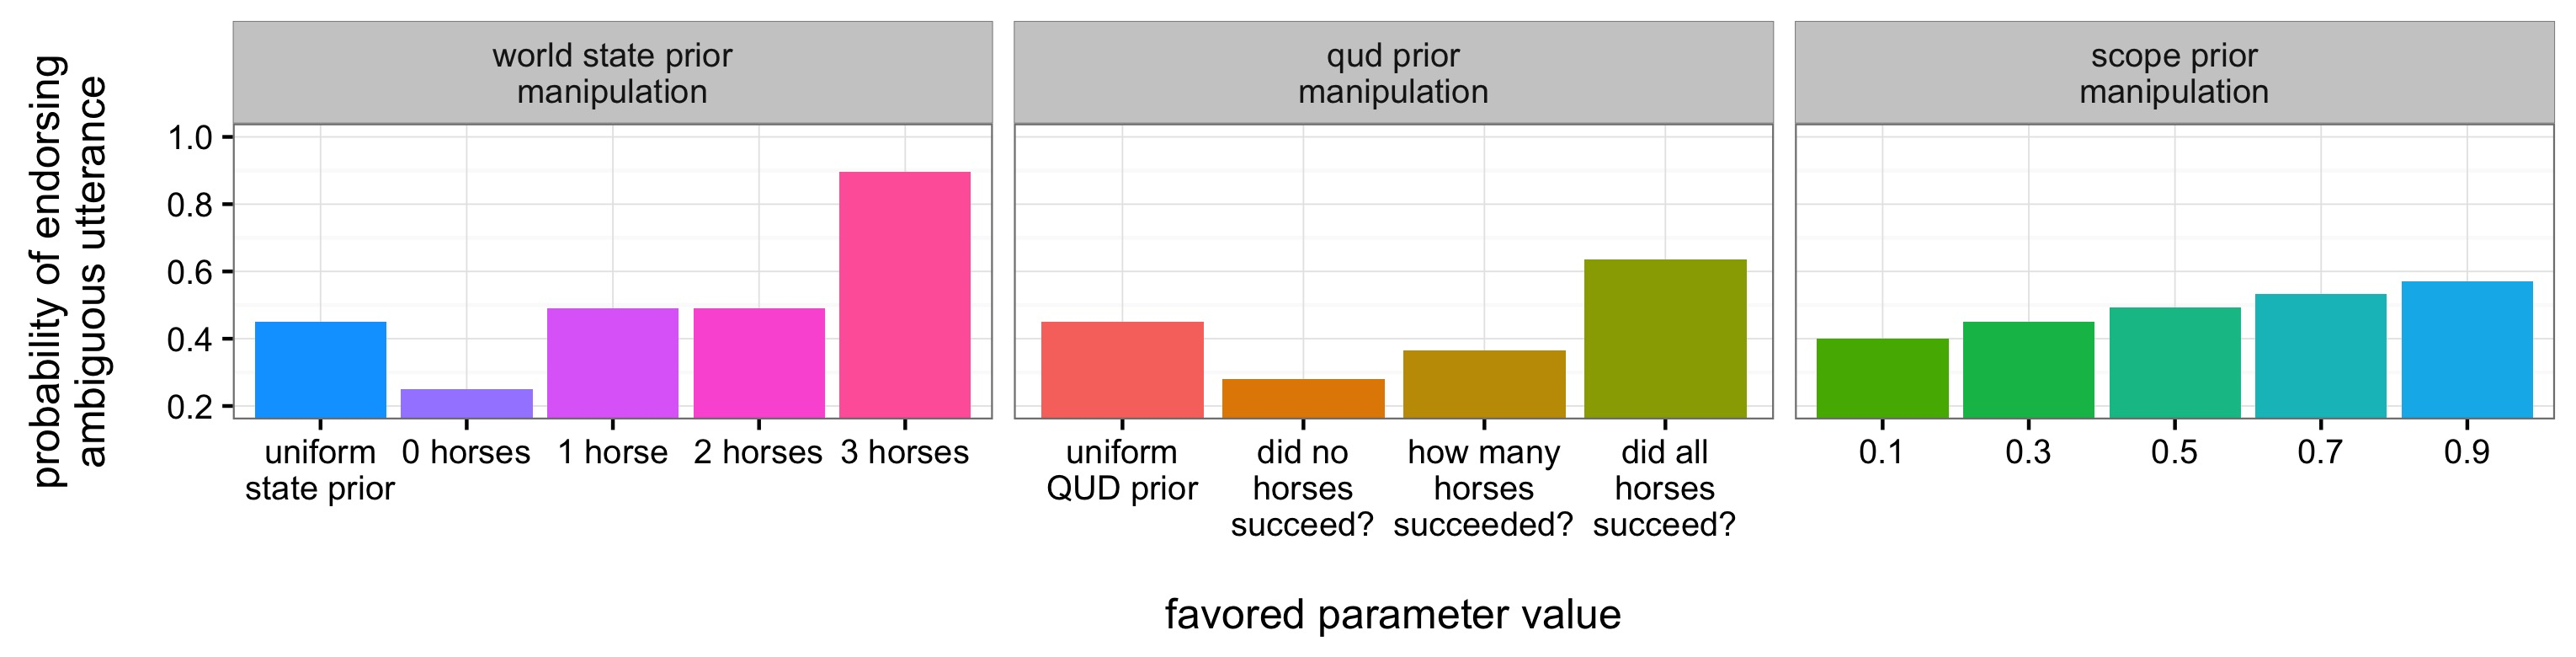
\includegraphics[width = \textwidth]{fig2.jpg}
\vspace{-15pt}
\caption{Model predictions for ambiguous utterance endorsement (e.g., \emph{Every horse didn't jump over the fence}) in a not-all scenario (e.g., two-out-of-three horses jump over the fence). Lower endorsement probability corresponds to less adult-like (i.e., more child-like) behavior. For the pragmatic variables (world state, QUD), the favored parameter value receives most of the prior probability weight ($P(favored) = 0.9$). For the processing variable (scope), the prior corresponds to how strongly the inverse scope is favored.}
\label{fig:graphs}
%\vspace{-10pt}
\end{figure*}

For the world state prior (Figure \ref{fig:graphs}, \emph{left}), we systematically favor specific world states by setting their prior probability to $0.9$; if a world state is not favored, it receives a prior probability of $0.1/3=0.033$. Holding the QUD and scope priors at their default values, we see a marked increase in endorsement of the ambiguous utterance in the not-all scenario as beliefs about horse success increase. Utterance endorsement is at its lowest ($0.25$) when prior knowledge suggests that horses are particularly unlikely to succeed at jumping; utterance endorsement is at its highest (i.e., most adult-like: $0.90$) when we believe horses are very likely to succeed.

Just as with the world state prior, we can systematically manipulate the QUD prior (Figure \ref{fig:graphs}, \emph{center}).  Favored QUDs receive a prior probability of $0.9$; other QUDs receive a prior probability of $0.05$. Holding the other priors at their default values, we see an increase in utterance endorsement from the \texttt{none?} (\emph{did no horses succeed?}; $0.28$) to \texttt{how-many?} (\emph{how many horses succeeded?}; $0.37$) to \texttt{all?} (\emph{did all horses succeed?}; $0.64$) QUDs. 
The model predicts the most adult-like behavior when the QUD concerns whether all the horses succeeded. 


Finally, for the binary scope prior (Figure \ref{fig:graphs}, \emph{right}), we systematically manipulate the prior probability of \texttt{inverse} from $0.1$ to $0.9$. Holding the other priors at their default values, we see a monotonic increase in utterance endorsement as the probability of \texttt{inverse} increases. At its most adult-like, the model predicts an endorsement probability of $0.57$ when the prior probability of \texttt{inverse} is at its highest ($0.9$)---at its \emph{lowest} (0.1), endorsement only drops to $0.4$.
%and note it only drops to $0.40$ when the prior probability of \texttt{inverse} is at its lowest ($0.1$).
%Utterance endorsement goes up the more the inverse is favored.  We see the most utterance endorsement probability at inverse = .9, ($P_{S_{2}} = .5716$).  And we see the least utterance endorsement at inverse = .1, ($P_{S_{2}} = .3999$)  

To summarize, the world state and QUD priors have a more dramatic impact on utterance endorsement than the scope prior.  There are two main reasons for this. 
First, for the world state prior, when expectations favor success (i.e., $w=3$), the ambiguous utterance is maximally informative regardless of the scope interpretation it receives: \texttt{amb} communicates to a listener that prior  expectations do not hold 
%LSP: explain this a touch more
(i.e., \textit{\textbf{None}/\textbf{Not all} of the horses succeeded} goes against the expectation that all three horses would succeed). So, \texttt{amb} is particularly useful for communicating about the \emph{a priori} unlikely not-all world states that appear in the experimental scenarios. 
Second, for the QUD manipulation, when \texttt{all?} is favored, 
 either interpretation of \texttt{amb} fully resolves the QUD: whenever \texttt{amb} is true (i.e., whether \textbf{None} or \textbf{Not all} the horses succeeded), it is not the case that all the horses succeeded. A pragmatic speaker recognizes the utility of \texttt{amb} as an answer to \texttt{all?} in a not-all world state, irrespective of the intended scope interpretation.


\begin{figure}[ht]
\centering
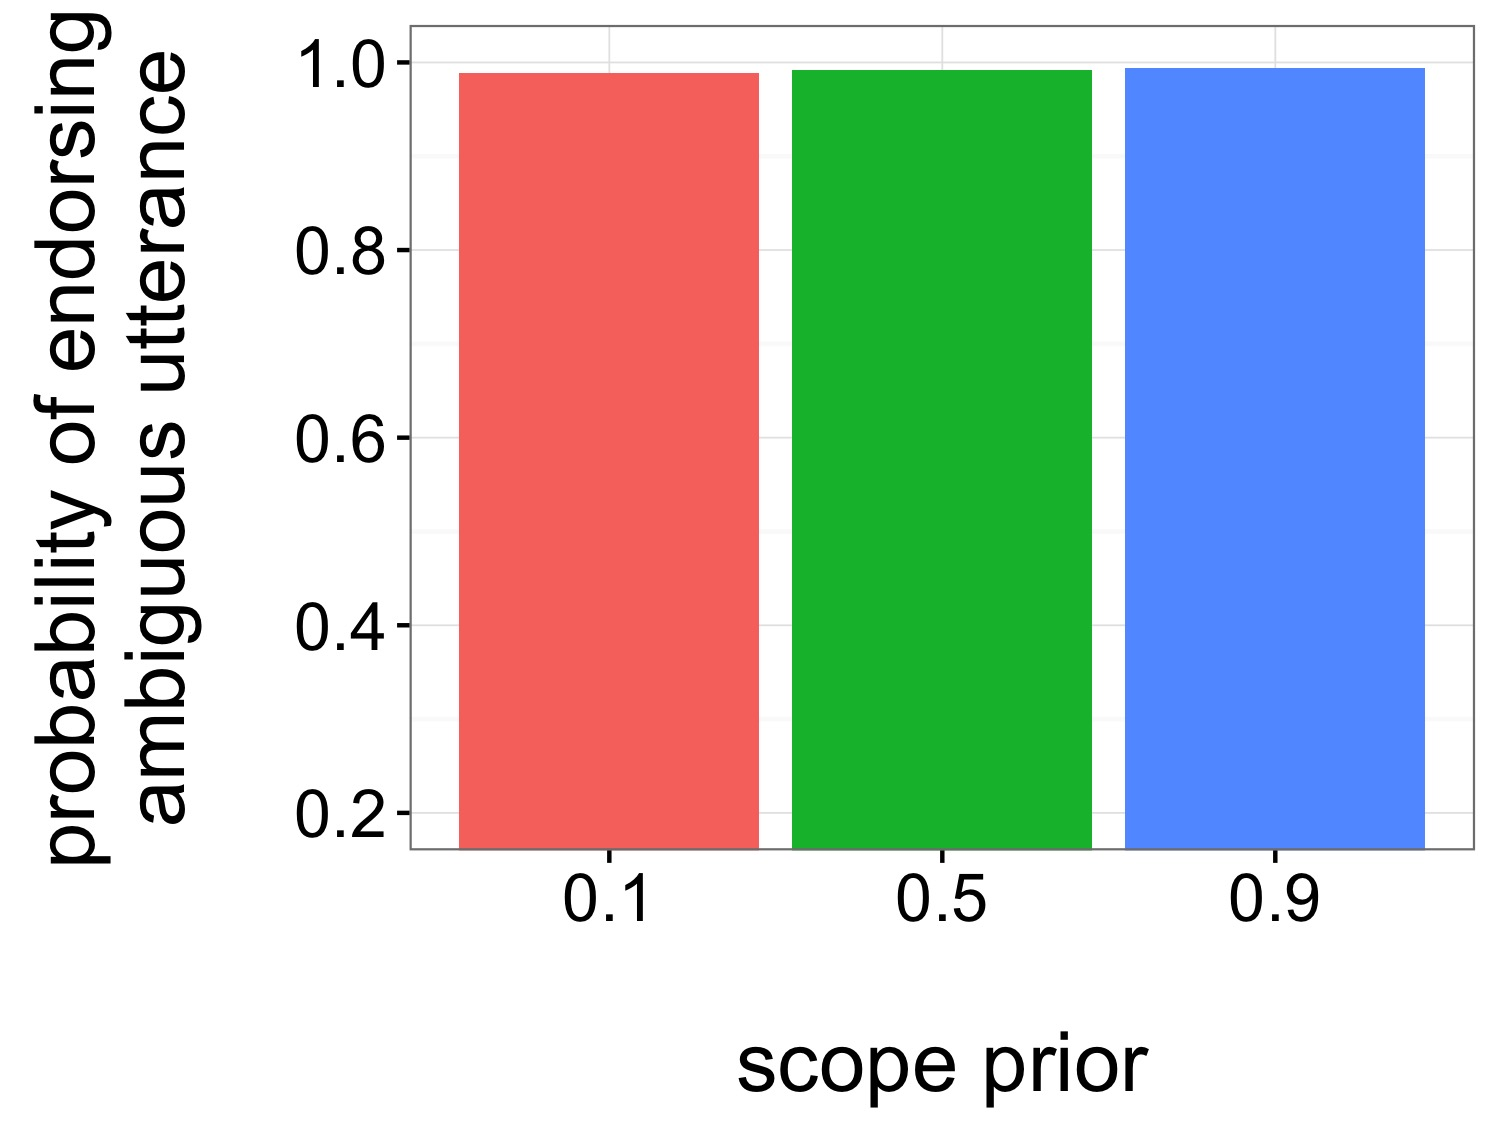
\includegraphics[width = 0.29\textwidth]{fig3.jpg}
\vspace{-5pt}
\caption{Model predictions for ambiguous utterance endorsement when optimal world state ($w=3$) and optimal QUD (\texttt{all?}) are favored ($P(favored) = .9$).}
\label{fig:interaction}
\end{figure}

So far, we have considered independent manipulations to the factors of interest. Figure \ref{fig:interaction} shows the interaction of all three factors for utterance endorsement when $w=3$ and \texttt{all?} are favored.
Here we see the additive effects of the world state and QUD priors; together, they lead to near-total endorsement of the ambiguous utterance. We also see more clearly the relatively small contribution of the scope prior, where changing the prior probability of \texttt{inverse} from $0.1$ to $0.9$ leads to just a $0.01$ increase in endorsement probability.  Thus, we see how the priors on the pragmatic  factors overwhelm the processing scope prior. When the optimal (i.e., optimal for endorsement) QUD and world state are favored, even when \texttt{inverse} is highly inaccessible (i.e., $P(\texttt{inverse}) = 0.1$), we still predict massive utterance endorsement ($0.99$).



\section{Discussion}

%% first takeaway = pragmatic factors overwhelm processing factors when pitted against each other
Our model of ambiguity resolution qualitatively captures the changes in children's utterance endorsement from the experimental literature;
our results suggest that when it comes to understanding non-adult-like behavior in the TVJT, there is a stronger role for the pragmatics of context management (as realized in priors on world state and QUD) than for grammatical processing (as realized in the prior on scope interpretations), although there is likely a role for both. 
So, the observed failure of children to endorse scopally-ambiguous utterances in not-all scenarios likely stems more from children's beliefs about the world of the experiment (e.g., whether horses are \emph{a priori} likely to succeed) and about the topic of conversation (e.g., whether the conversational goal is to determine if all the horses succeeded), than their inability to grammatically derive the inverse scope interpretation in real time.  
Indeed, our model predicts the highest rates of utterance endorsement to occur when resolving the scope ambiguity is \emph{irrelevant} for communicating successfully about the not-all world---that is, when expectations favor total success (i.e., $w=3$), or when the QUD asks if \texttt{all?} of the horses succeeded. In either case, both scope interpretations serve to inform a listener, either that the \emph{a priori} likely $w=3$ isn't true or that the answer to the \texttt{all?} QUD is \emph{no}. 

% now let's talk bigger takeaway w.r.t experimental design
These results also underscore the need for well-defined mapping hypotheses from observed experimental behavior to the psychological processes they inform, particularly for the sophisticated reasoning that occurs in tasks like the TVJT. 
In our brief review of the experimental literature, we were careful to point out 
alternative interpretations of the various experimental manipulations and their  potential, unintended pragmatic consequences.
At the very least, we hope to have demonstrated that utterance endorsement is not simple. A TVJT participant must reason recursively about the potential  informativity of the utterance, attending to knowledge about the world of the experiment and the likely topic of conversation. That children stumble when attempting to perform these complex recursive inferences isn't so surprising. 
We suggest that a plausible source of differences in child and adult behavior on the TVJT is  children's inability  to successfully manage pragmatic information. We therefore propose to move the discussion away from the \emph{fragility} of accessing inverse scope in children as a grammatical processing deficit and toward the \emph{complexity} of behavior that scope interpretations require.

%Discuss how we don't know from the experimental literature the exact setting of the knobs of the model.  So we're going to propose specific experiments to assess these explicitly and see what their values are.
 In addition to formalizing the pragmatics of ambiguity resolution in context, our results also motivate future experimental investigations that explicitly measure children's (and adults') expectations about the world and topic of conversation. We saw how past experiments did not completely deconfound the relevant factors. Perhaps the most straightforward way of testing these factors' effects is to \emph{measure} the prior knowledge that participants bring to bear in the TVJT.
 %and/or more explicitly manipulate this contextual knowledge.  
 %  One suggestion might be establishing a concern for the puppet (the QUD) that is in opposition to the listener's (or puppets) knowledge of the horses.  For example, maybe the conversation is about 0 horses making it over because a character in the story placed a bet on this outcome.  But we also know from the story that horses are good a jumping (the bet was risky).   
 %% and then we can model these to get a more quantitative fit to participant behavior
 These explicit measurements of pragmatic context can then form the basis of future modeling studies in this framework that could quantitatively match the behavioral results.
 
 %We know from Lidz (2002) that we can turn children into adults.  Perhaps using these turned adults would be a good paradigm to test the impact these pragmatic factors have on utterance endorsement, since we can more easily measure adults knowledge of the world/conversation than children's knowledge of these variables.
 
%With adults, it might be easier to access what they believe the conversation is about.  Since we can turn adults in to children \cite{lidz2002children}, perhaps we could turn them back into adults with manipulations to these contextual factors.  This would allow us to assess how a listeners (adults) beliefs about the contextual factors would influence their access to the inverse scope interpretation.   

More generally, our results provide the foundation for more complete theories of the developmental process underlying scope ambiguity resolution. Children's relative lack of experience managing world and conversational knowledge likely contributes to their sensitivity to the experimental context.
%- more relative information gain is happening during the experiment.
% - when children get information in the TVJT, this information will 
%\gcs{we'll have to say something a bit more coherent}
%%% Lidz-style pithy closing statement to the effect of "at five, you're semantically solid but pragmatically still developing"
In short, five-year-olds may know the right interpretation, but they're still figuring out whether it's the best answer in the context of the experimental conversation. 
 








%Just testing two column effect with figures
% \begin{figure}[H]
% 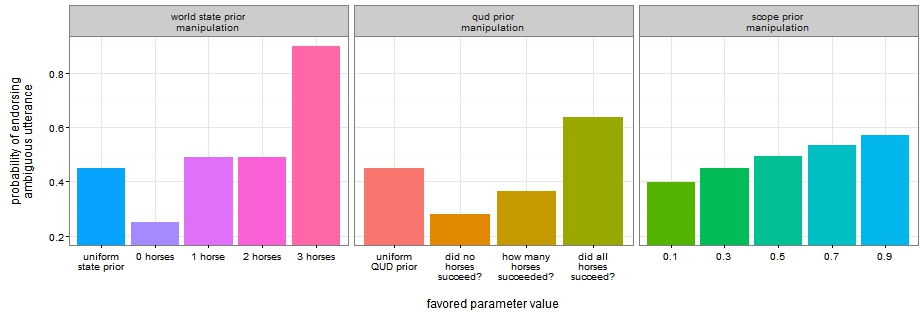
\includegraphics[width = \textwidth]{little-plot.jpeg}
% \label{fig:graphs}
% \vspace{-2em}
% \caption{Model predictions: Probability that a pragmatic speaker would endorse an ambiguous utterance (i.e., \emph{Every horse didn't jump over the fence}) in a scenario where one out of two horses did. Lower probability of endorsement corresponds to less adult-like (i.e., more child-like) behavior. For the contextual variables (world state, QUD), the favored world state or QUD is the one that has most of the prior probability weight. For the grammatical processing variable (scope), the prior corresponds to how strongly the inverse scope is favored.
% }
% \end{figure}

%\section{Acknowledgements}


\bibliographystyle{apacite}
\setlength{\bibleftmargin}{.125in}
\setlength{\bibindent}{-\bibleftmargin}

\bibliography{MyBib}

\end{document}


\newpage


\section{extra bits}

\subsection{backgrond}

in the TVJT by making the QUD explicit. 
\gcs{we need more information about Gualmini 2004. How was the QUD manipulation effected? I would try to model this on the discussion of Musolino and Lidz above: first the manipulation, then the effect, then our interpretation of the manipulation} 
\lsp{seconded on the structure suggestion. My best guess right now below.}


[manipulation: make QUD explicit? e.g., ``Did the troll deliver all the pizzas?''. Two puppet utterance options: \textit{The troll didn't deliver/lose some pizzas.} in a scenario where there are XX pizzas total and the troll delivered YY. 

Surface scope: It's not the case that he delivered/lost some. (implication: \textbf{None} delivered/lost)

Inverse scope:  There are some that he delivered/lost. (implication: \textbf{Not all} delivered/lost)

QUD answers for ``Did the troll deliver all the pizzas?'': 

Surface-deliver (delivered none) = No.

Inverse-deliver (delivered not all) = No.

Surface-lose (lost none = delivered all) =  Entailment: Yes

Inverse-lose (lost not all = delivered some?) =  Entailment:  Probably not all delivered either.

Upshot: surface-deliver and inverse-deliver are both good answers to QUD, especially when compared to surface-lose and inverse-lose.  But surface-lose is better than inverse-lose.
]

[effect:
\lsp{example numbering got messed up, so need to check this}
For (5) [utterance-lose?], only the surface interpretation [surface-lose] perfectly answers the QUD 
(even if it requires some entailment) 
so children will favor that interpretation over the inverse interpretation [inverse-lose].  Just as predicted, children who heard (4) [utterance-deliver?] accepted the utterance 90\% of the time, whereas children who heard (5) [utterance-lose?] only accepted the utterance 50\% of the time \cite{gualmini2004some}.
(So we're comparing inverse-deliver vs. inverse-lose?)
]

[interpretation: 
manipulated QUD (made a specific one salient).
Did we also manipulate the world expectations at all, by highlighting the success rate?
]


Gualmini (2008) reports on the experiment from Gualmini (2004) which involved two conditions, one where children heard an utterance like (4) and another where they heard an utterance like (5):

\ex. 
\a. The troll didn’t deliver some pizzas
\b. the troll didn’t lose some pizzas

\noindent These were uttered by a puppet in a context where the salient QUD was:


\ex. Did the troll deliver all the pizzas?

\noindent We can paraphrase the surface and inverse interpretations of (4) and (5):


\ex.
\a.surface: the troll didn’t deliver any pizzas
\b. inverse: there are some pizzas the troll didn’t deliver

\ex.
\a. surface: the troll didn’t lose any pizzas
\b. inverse: there are some pizzas the troll didn’t lose

Like past experiments, the surface interpretations were false and the inverse interpretations were true.  In the case of (4), both interpretations entail a `no' answer to the QUD in (6).  In (5), however, only the surface interpretation, (5a), entails an answer to the QUD (in this case, a `yes' answer).  The Question-Answer requirement predicts that children will accept (4) more than (5). They will abide by the principle of charity in (4) when both interpretations answer the QUD, thus accessing the inverse interpretation.  For (5), only the surface interpretation perfectly answers the QUD so children will favor that interpretation over the true inverse interpretation.  Just as predicted, children who heard (4) accepted the utterance 90\% of the time, whereas children who heard (5) only accepted the utterance 50\% of the time \cite{gualmini2004some}.


\subsection{model}

As for the other two priors, we systematically adjust these priors across ranges that cover a uniform state, and a favoring of each value.  For world state we consider the uniform, $s_0 = s_1 = s_2 = s_3 = .25$, and priors that favor a particular state where the favored state is $w_favored = .7$ and unfavored world states are set to, $w_unfavored = .1$.  Similar with QUDs, we have the uniform state, $q_many = q_all = q_none = (1/3)$, and the favored states where the favored state $q_favored = .8$ and the unfavored states get, $q_unfavored = .1$.    

The second speaker level is where this RSA model departs from models past.  Again, the data we are modeling is not `pure' utterance comprehension data.  The participants of the TVJT have access to the world state.  So we invert the pragmatic listener in the pragmatic speaker, and draw a marginal distribution over utterances given a world state:

\begin{equation}
P_{S_{2}} (u | s) \propto \ P_{L_{1}} (s, v, q | u)
\end{equation}



We interpret the resulting probabilities over utterances to be a kind of ‘endorsement’ probability, where a relative shift in the probability of an utterance indicates a shift in the likelihood of this speaker endorsing the utterance in that world state.   

We can consider the rather ubiquitous utterance, “every horse didn’t jump over the fence,” when concertizing the variables and levels of the model.  To represent the extra-linguistic variables, we consider two in particular that have been implicated in allowing for children to access the inverse scope interpretation: world knowledge and conversational knowledge \cite{viau2010priming,gualmini2004some}.  World knowledge represents how much the listener knows about the world state, where we consider world states where zero horses made it over the fence, $s_0$, where one horse made it over the fence, $s_1$, and where all the horses made it over the fence, $s_2$.  Conversational knowledge represents the listener's knowledge of the QUD of the discourse.  This amounts to a prior probability distribution over QUDs.  We consider three QUDs in particular for the above utterance: ``how many horses made it over?" (`many?') ``did all the horses make it over?" (`all?') and ``did none of the horses make it over?" (`none?').  For the linguistic variable, or scope variable, we adjust the prior weight on which scope interpretation is favored by the listener.  In this way, we computationally capture a `processing' preference for one interpretation or the other.

The base layer of RSA models is the literal listener.  The literal listener draws a probability distribution over world states, given the literal semantics of the utterance with an intended scope interpretation said within a given conversational context:

\begin{equation*}
P_{L_{0}} (s | u, v, q) \propto  \ [\![u]\!]^{v,q}(s) \cdot P(s)
\end{equation*}

\noindent $P_{L_{0}} (s | u, v, q)$ is the probability distribution the literal listener draws over world states, given fixed values for all the other variables.  

The first speaker chooses an utterance given the distribution drawn by the literal listener.  We consider two utterances that the speaker can choose from, the scopally ambiguous utterance ``Every horse didn't jump over the fence" and saying nothing (the `null' utterance).  Alternative unambiguous utterances would impact the results.  Although future work could consider adding other utterances into the model, we want to restrict our analysis to the three variables already mentioned. 
%want to say this better
`Informativeness' here is captured by how much a given utterance communicates about a world state.  As an example, if the speaker is in $s_2$, which utterance would leave the literal listener with the most probability mass on this world state?  In this case, the `null' utterance would because the scopally ambiguous utterance is false in this world state.   In the tradition of other RSA models, we use a soft-max decision rule for the speaker’s utterance selection. $\alpha$ here is an optimality parameter that controls how rational the speaker will be in utterance selection.  (Random  (Sutton and Barto, 1998) reference I’ve never read):

\begin{equation}
P_{S_{1}} (u | s, v, q) \propto  \ exp (\alpha \cdot log(L_{0}(s | u, v, q)))\\
\end{equation}

\noindent We've set $\alpha$ to 2.5, which makes the speaker fairly optimal (the speaker assigns very little weight to less informative utterances with this value).  

In line with other RSA models, a pragmatic listener inverts the speaker model with Bayes’ rule.  The uncertainty regarding the contributing variables is implemented into the model here.  The pragmatic listener will draw a joint probability distribution over scope assignment, world state, and QUD, given the speaker’s utterance. 

\begin{equation}
 P_{L_{1}} (s, v, q | u) \propto  \ P_{S_{1}} (u | s, v, q) \cdot P(s) \cdot P(v) \cdot P(q)
\end{equation}

\noindent Where $P(s)$, $P(w)$, and $P(q)$ are the priors over the two extra-linguistic variables, world knowledge and conversational knowledge, and the one linguistic variable, scope.  How do we decide how to set these variables? Past experiments lack measurements of the participants beliefs about these values.  With respect to scope, we suspect that humans have a slight preference for the surface interpretation (citation).  For this reason, the default values for are $v_surface = .7$ and $v_inverse = .3$.  As for the other two priors, we systematically adjust these priors across ranges that cover a uniform state, and a favoring of each value.  For world state we consider the uniform, $s_0 = s_1 = s_2 = s_3 = .25$, and priors that favor a particular state where the favored state is $w_favored = .7$ and unfavored world states are set to, $w_unfavored = .1$.  Similar with QUDs, we have the uniform state, $q_many = q_all = q_none = (1/3)$, and the favored states where the favored state $q_favored = .8$ and the unfavored states get, $q_unfavored = .1$.    

We systematically adjust these prior values in order to determine how each of them will impact the endorsement of the scopally ambiguous utterance in the next level, the second speaker.

The second speaker level is where this RSA model departs from models past.  Again, the data we are modeling is not `pure' utterance comprehension data.  The participants of the TVJT have access to the world state.  So we invert the pragmatic listener in the pragmatic speaker, and draw a marginal distribution over utterances given a world state:

\begin{equation}
P_{S_{2}} (u | s) \propto \ P_{L_{1}} (s, v, q | u)
\end{equation}

We interpret the resulting probabilities over utterances to be a kind of ‘endorsement’ probability, where a relative shift in the probability of an utterance indicates a shift in the likelihood of this speaker endorsing the utterance in that world state.   


\subsection{results}

%Figure 2 shows the interaction effects from the three variables.  We notice here as well that the `many’ QUD maximizes the impact of a scope prior manipulation.  Since this QUD asks for an individual world state as a response (as opposed to an aggregate of states answering the question) utterances with disjoint semantics will be more readily distinguished.

The interaction plot reveals how the priors on the contextual factors overwhelm the scope prior.  When the optimal (optimal for endorsement) QUD and world state are favored in the prior, even when the inverse is highly dispreffered (inverse = .1) we still see massive utterance endorsement ($P_{S_{2}} = .9104$).  This is also true when the sub-optimal QUD and world state priors are favored when the inverse is highly preferred (inverse = .9); ($P_{S_{2}} = .3423$).  These interaction results can depend on how many world states we consider, which QUDs we consider, and how disjoint the scope interpretations are.  In the right context, however, these results suggest that contextual factors could easily counteract any difficulty in accessing the inverse scope.      

% \begin{figure}
% \centering
% 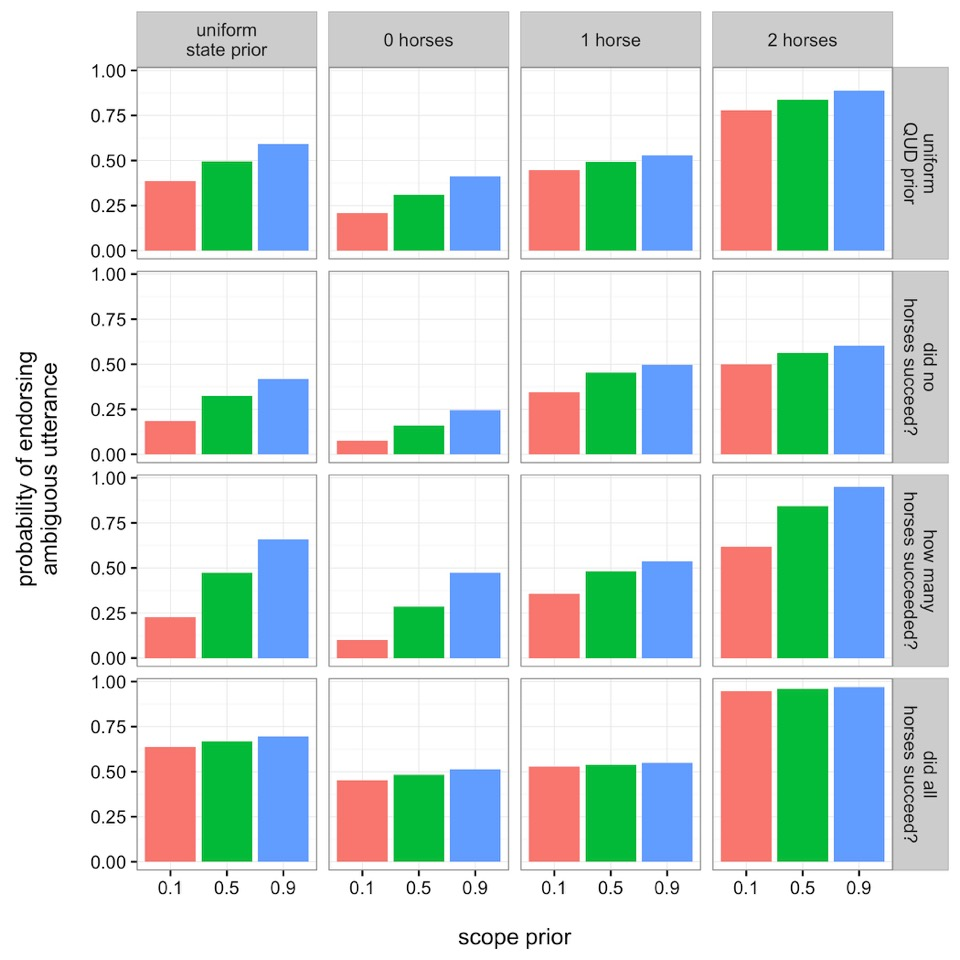
\includegraphics[height=12cm]{big-plot.jpeg}
% \label{fig:graphs}
% \caption{Interactions between manipulated parameters.} 
% \end{figure}

We also notice that the impact of the QUD manipulation and the world state manipulation are additive.  When world state 2 and the `all?’ QUD are favored, we see endorsement probabilities close to 1 across all of the scope priors. 

(Hmmm, is there more data we can get from this graph?)   

How much detail to go into with explaining model results.


The first is that the two scope interpretations are not disjoint in their semantics: both interpretations truthfully describe a scenario in which no horses jumped over the fence. \gcs{why should this matter?} 
%We see a more dramatic impact from a scope manipulation in the model when we use an utterance whose interpretations are perfectly disjoint (like ``the detective didn’t find two guys”). 
Another reason for the low impact scope manipulation concerns the QUDs in the model.  The QUD, ``did all the horses jump over the fence” disambiguates the scopally-ambiguous utterance ``every horse didn’t jump over the fence” since both interpretations perfectly answer the QUD. \gcs{why should this matter?} When we just use the `many’ QUD in the model, the scope manipulation is more impactful (numbers). \gcs{why?}

\kj{world state explanation}

When the prior favors the 0 world state, the pragmatic speaker doesn't endorse the ambiguous utterance very much (number).  This is largely due to the 'none?' QUD, where the null utterance gets more weight on the 'no' side of the partition because it is 'true' in all world states.  This will increase `null' endorsement drastically when the 0 world state is favored and we end up in world state 2.  When you get ride of the 'none?' QUD, the endorsement moves up to (higher than above), but it is still pretty low.  This is largely because the surface scope is true in this world state, and is only true in this world state.  So when you heavily favor the 0 world state, you are giving more weight to an interpretation that is already very strong (and has 0 weight in world states 1 and 2).  

\kj{general note for clarity: The size principle will always have it so the the stronger utterance is endorsed if all utterances are true in the world state - all things being equal.  In our case, the size principle gets exaggerated when world state 3 is favored. (I'm always talking about endorsing in world state 2 (or 1 cause its identical)}  

What happens when world state 3 is favored?  This is an interesting case. You get massive endorsement of the ambiguous utterance (numbers).  Why is this? It's largely a matter of relative weight in world state 2 compared to the null's weight in that world state. Since the null is `true' in every world state and is the only utterance that is 'true' in world state 3, when we normalize in the pragmatic listener given an utterance, world states 0,1,2 shrink massively in the null compared to in the ambiguous utterance.  So the weight for world states 1 and 2 in the ambiguous utterance are now much higher than those shrunken probabilities in the null. When you consider world states 1 and 2 now, those probabilities in the pragmatic listener are going to be much higher than the corresponding probabilities in the null.  When we get to the pragmatic speaker, they will be reasoning about the pragmatic listener in world state two, and give strong endorsement.

\kj{QUD explanation}

There is a simple heuristic (mathematically justified) that will inform us as to the strength of the utterance endorsement with respect to QUD prior manipulations. The more vague \kj{I originally was using `ambiguous' here, but I think `vague' is more accurate} a QUD makes the utterance, the less endorsement we get.  The ranking of the QUDs by how vague they make the utterance are 1. 'none?' 2 'many?' 3. 'all?'.  'all?' technically disambiguates the utterance, making it perfectly `not vague', so this QUD maximizes endorsement in the QUD manipulations.  'none?' makes the utterance more vague than 'many?' because the inverse in 'none?' gets weight in world state 3 (so it `smears' that probability over more world states, maximizing the number of world states that the utterance is 'true' in, making it more vague than 'many?').






\end{document}

%stats to get